% !TeX spellcheck = en_GB
\documentclass[10pt,a4paper,kul]{kulakarticle} %options: kul or kulak (default)

\usepackage[utf8]{inputenc}
\usepackage[english]{babel}
\usepackage[T1]{fontenc}
\date{2024 -- 2025}
\address{
	Engineering Technology\\
	Distributed Systems\\
	Bert Lagaise
}
\title{Report Final Project}
\author{Robbe Decapmaker, Wout Lyen, Lander Van Loock, Kobe Michiels}

\usepackage[backend=biber,style=ieee, natbib=true]{biblatex} % Use a proper package for managing bibliography
\addbibresource{ugh.bib}

\usepackage{hyperref}
\usepackage{graphicx}
\usepackage{amsmath, amssymb, amsthm}
\usepackage{siunitx}
\usepackage{flafter} 
\usepackage{pdfpages}
\usepackage{pgfplots}
\usepackage{caption}
\usepackage{subcaption}
\usepackage{multicol}
\usepackage{floatrow}
\usepackage{float}


\begin{document}
	\maketitle  
	\section*{Introduction}
		This report presents an overview of a modern web-based retail platform specializing in the sale of bicycles equipped with RGB LED strips, a product that blends functionality, safety, and aesthetic appeal for urban and recreational cyclists. The web-shop is designed to deliver a seamless shopping experience while leveraging a robust, distributed architecture deployed on Microsoft Azure.\\
		By operating across various administrative and geographic boundaries, the system ensures high availability, scalability, and resilience. The use of Azure’s global infrastructure enables efficient resource allocation, data redundancy, and compliance with regional data protection regulations. This report explores the technical design, deployment strategies, and operational considerations of the platform, with a focus on how distributed cloud services support the business’s scalability and cross-regional presence.

	\section{General Architecture}
		\begin{figure}[h]
			\centering
			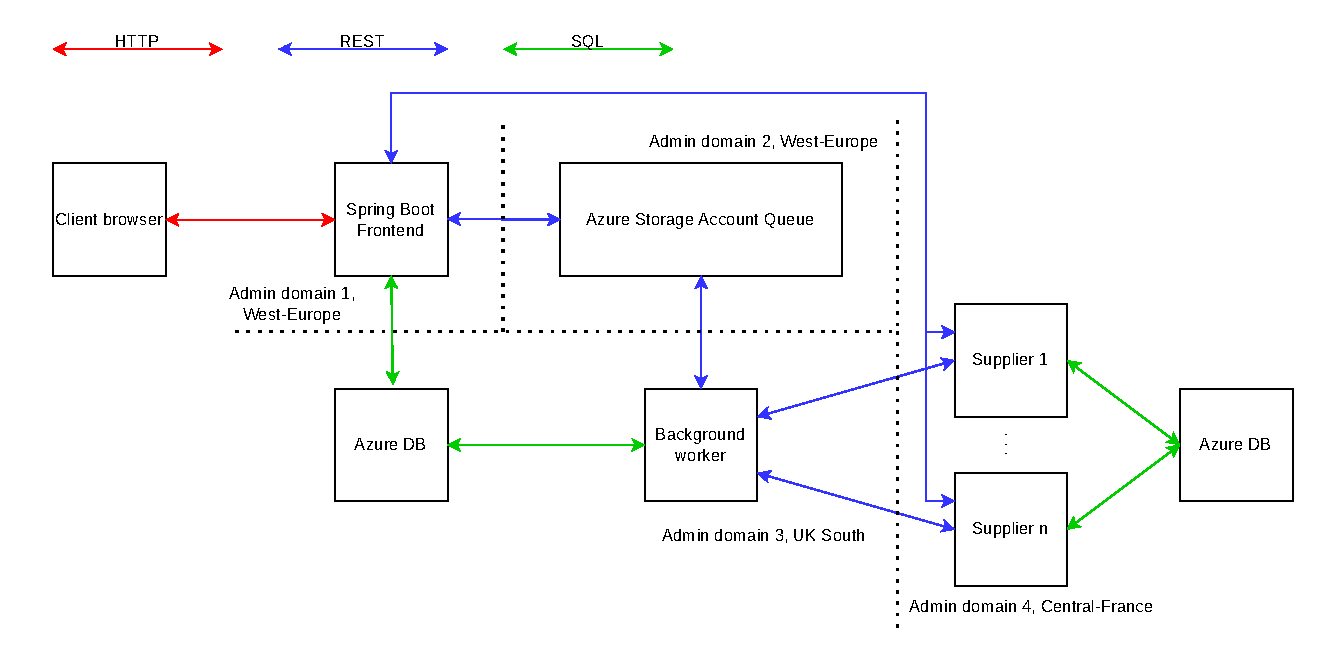
\includegraphics[width=1\linewidth]{images/arch}
			\caption{General overview of the architecture}
			\label{fig:arch}
		\end{figure}
		
	
	\section{Front-end Details}
	
	\section{Broker Details}
	
	\section{Supplier Details}
		Although the suppliers are an indirect part of the web-store, they do take part in the distributed commit. Because of this, careful thought had to be put in to ensure proper processing of an order. 
		\subsection{Design}
			A supplier is essentially a PHP API with a number of endpoints useful for retrieving information about products and orders. As well as making a distributed commit of-course. On a high level, the following endpoints are available:
			\begin{description}
				\item[list\_products] provides information such as id, name, description, stock and an image url for all products. 
				\item[reserve] provides a starting point for the distributed commit. It acts as a \emph{request} operation. It expects information such as a global order id, other partaking parties and of-course product information. 
				\item[show\_reserve] provides information about reservations currently filed by a user.
				\item[commit] provides a way to confirm a reservation. It acts as a\emph{commit} operation. It just needs to know which global order id needs to be committed. 
				\item[show\_commit] provides information about the commits currently filed by a user.
				\item[rollback\_reservation] provides a way to cancel a reservation. It acts as an \emph{abort} operation. It just needs to know which global order id needs to be reverted. 
				\item[rollback\_commit] provides a way to cancel a commit. It is not part of the standard two-phase commit but can be used for cancelling confirmed orders. 
				\item[cleanup\_reserve] provides a way for users with extra privileges to clean-up stale reservations in case they have been abandoned by the broker. 
				\item[transaction\_check] provides a way for users with extra privileges to request the status of any global order id, it acts as a part of the mechanism to communicate among suppliers in case of a broker failure. 
				\item[check\_other\_sup] provides a way for users with extra privileges to perform a synchronisation of waiting reservations with their respective peers.  
			\end{description}
			
			In order to secure these endpoints, we protected them with SSL so there would be no unencrypted data on the wire. This was done using free \emph{Let's Encrypt} certificates which renew automatically. Another level of protection is the API-keys which are required to talk to a supplier. These API keys are registered in a  database and are associated with an entity name and privilege level. This way, ordinary brokers can't perform the same tasks as an admin user. This helps to ensure critical actions such as clean-up and synchronisation are only performed by the right entity. Another layer of protection is the Nginx web-server which serves the PHP API to the outside world. It is configured to protect any assets which contain sensitive information, only allowing traffic to the PHP and picture assets. 
			
			In order to help avoid inconsistency in the suppliers, a lot of effort was put into making sure a malformed input has no effect on the transactions. This is done by checking the contents of a request to see if it contains the right data for performing the requested operation. Furthermore, if something does manage to slip through the cracks, the PHP works with DB transactions. Essentially, when a critical section of the code is reached, an SQL transaction is started. Following this, all operations are performed on the database and finally they are committed when everything is successful. If something goes wrong in the critical section however, the entire transaction gets rolled back. 
			
			In the event of a crashed machine which partakes in the distributed commit, nobody can be exactly sure who received what message (depending on which machine failed). That is why the callback mechanism was introduced in the suppliers. When a reservation gets made, the broker is responsible for adding information about which machines partake in the transaction  (suppliers and broker). Because the broker supplies this info, we have the flexibility to perform a commit which can involve a varying amount of suppliers. Essentially, the customer can choose not to buy a battery kit. This would result in the bike and RGB supplier knowing not to communicate with the battery supplier. When communication is needed, the suppliers can take advantage of the \emph{transaction\_check} and \emph{check\_other\_sup} routes. In general, there can be a cron which periodically calls the latter route of all suppliers to regularly facilitate communication between suppliers and brokers. 
			%TODO:
			%% security: SSL
			%% security: API key, with different levels of access
			%% PHP for extra points
			%% Same code base, different env variables
			%% Nginx
			%% The whole setup with transactions on the DB
			%% Supplier callback mechanism
			%% Endpoints, and what they can do
			%% Error handling 
			%% Input validation
			%? Distributed commit from the point of view of a supplier
			%? Future work: Transition to prepared statements for SQL injection mitigation
		
		\subsection{Deployment}
			\autoref{fig:supplier} shows the schematic representation of the suppliers' deployment. Each gets their own VM and DB, this is to emphasise the fact that they run fully separate from each other. One does notice the fact that the DBs are all hosted in the same Azure structure. This does not mean that this has to be done for deployment, it just means we saved some time and money by only setting up one Azure DB instance. The separation between different suppliers data is still ensured. All VMs also run the exact same code, the way they differentiate which DB to talk to for example is by taking advantage of environment variables. In this case, they are injected by PHP-FPM which can simply be configured using one configuration file on each VM. 
			\begin{figure}[h!]
				\centering
				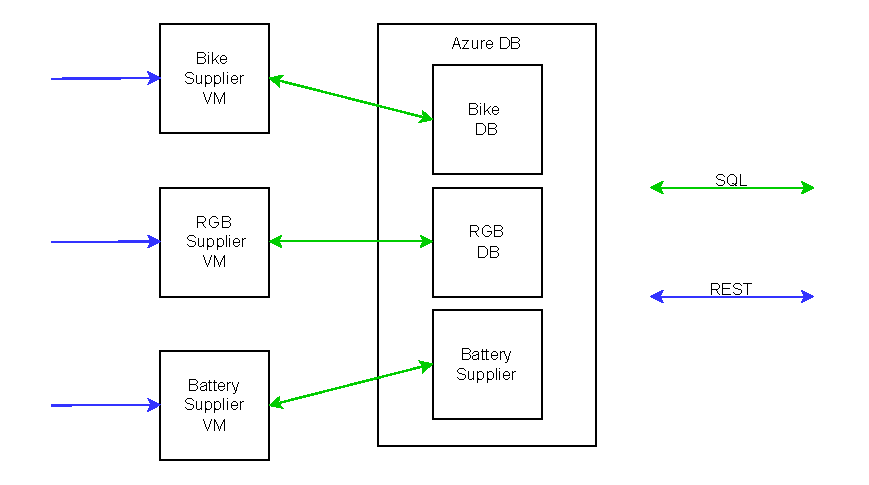
\includegraphics[width=0.7\linewidth]{images/supplier}
				\caption{Detailed architecture of the suppliers}
				\label{fig:supplier}
			\end{figure}
		
	\section{Load testing}


	\section{Cost overview}
	
		\subsection{Suppliers}
			The supplier infrastructure supporting the web-shop is designed with cost-efficiency in mind, particularly during the initial phases of operation. This infrastructure relies on three virtual machines (VMs) hosted on Microsoft Azure, along with a MySQL database, all of which initially operate within Azure's free tier offerings.\\
			Each of the three VMs benefits from Azure’s free tier, which provides up to 750 compute hours per month. This allocation is sufficient to run one VM continuously or distribute usage across multiple VMs with careful scheduling. Once the 750-hour limit is exceeded in any given billing cycle, the VMs automatically transition to Azure’s lowest-cost paid tier. This tier continues to offer basic compute capabilities at a minimal cost, ensuring that the infrastructure remains economically sustainable even under moderate usage.\\
			Similarly, the MySQL database is provisioned under Azure’s free tier for managed databases. It remains free until it exceeds the usage limits defined by the 750-hour threshold. Upon reaching this limit, the database instance shifts to the lowest available pricing tier, maintaining essential functionality while controlling costs.\\
			By leveraging Azure’s free tier and its seamless transition to cost-effective paid options, the supplier infrastructure is able to support operational demands with minimal upfront expenditure. This approach allows for scalability and consistent performance while keeping cloud resource costs predictable and manageable as usage grows.
	
\newpage
  \section{Extra information}
  \begin{itemize}
    \item Robbe Decapmaker - R0848369
    \item Wout Lyen - R0887788
    \item Lander Van Loock - R0886277
    \item Kobe Michiels - R0848543
  \end{itemize}
  

\end{document}

